% ######################################################################################################################
%         Balances
% ######################################################################################################################

\chapter{Balances}
\label{ch:Balances}

\paperbox{
    This chapter is derived from parts of the peer-reviewed open-access publication:
}{\paperpppp}{
    All text and figures in this chapter were created by Lucas Czech.
    Mathematical decisions of the balances and taxon weighting scheme emerged from discussion with Justin Silverman.
}

% \todo{distance measures, nhd, simulations, mantel test}

% ######################################################################################################################
%         Background and Motivation
% ######################################################################################################################

\section{Background and Motivation}
\label{ch:Balances:sec:Motivation}


% \subsection*{Phylogenetic ILR transform and Phylofactorization}
% \label{sec:MaterialsMethods:sub:Balances}

The concepts and methods presented in the previous Chapters~\ref{ch:Visualization} and \ref{ch:Clustering}
resemble two recent approaches for analyzing phylogenetic data:
the Phylogenetic Isometric Log-Ratio (\emph{PhILR}) transformation and balances \cite{Silverman2017},
as well as Phylogenetic Factorization (\emph{Phylofactorization}) \cite{Washburne2017a}.
These methods use a tree inferred from the OTU sequences of the samples (instead of a fixed reference tree),
and annotate the abundances of OTUs per sample on the tips of this tree (instead of placement masses on the branches).
The methods use these data to draw conclusions about compositional changes of OTU abundances in clades of the tree in different samples,
as well as relationships of per-clade OTU abundances with environmental meta-data variables.
See \secref{ch:Foundations:sec:SequenceAnalysis:sub:OTUs} for details on OTU clustering of metagenomic samples.

% The PhILR transform computes a \emph{balance} between the OTU abundances
% in the two subtrees below a given inner node of the tree...
% two disjoint sets of tips (for example, the two subtrees below a given inner node of the tree).

In both of these approaches, a \emph{balance} between OTU abundances in two subtrees of the underlying tree is computed.
This is a measure of contrast that expresses which of the two subtrees comprises more OTUs in a sample.
In the PhILR transform  \cite{Silverman2017}, these balances are computed
for the two subtrees below each inner node of a rooted binary tree,
while ignoring abundances in the respective remainder of the tree.
In Phylofactorization however, these balances are computed
for the two subtrees that are induced by the splits/edges of the tree \cite{Washburne2017a}.
This is highly similar to the concept of edge imbalances 
that we introduced in \secref{ch:Foundations:sec:PhylogeneticPlacement:sub:PlacementProcessing:par:EdgeImbalances}.
Note that despite sharing a similar name and exhibiting conceptual similarities,
balances and edge imbalances are distinct approaches that should not be confused.
We later discuss respective similarities and differences in more detail.

Furthermore, we remark that the \emph{Balance Trees} method \cite{Morton2017} employs analogous concepts
by calculating the balance of nodes using the isometric log-ratio of OTU abundances.
However, instead of using a phylogenetic tree, it assumes any binary partitioning of the OTUs,
e.\,g., obtained from a UPGMA clustering \cite{Legendre1998} of the OTUs based on a meta-data feature.
These nodes thus correspond to specific meta-data values,
again allowing for statements about the changes in OTU abundances that occur with changing environmental variables.
%value thresholds that separate distinct samples.
% As this is not directly applicable to phylogenetic placements,
As we already have a binary partitioning in form of the reference tree,
we do not further consider the Balance Trees approach here.

In this and the following chapter, we present adaptations of the PhILR transform (balances)
and of Phylofactorization to phylogenetic placement data.
The main adaptation step consists in placing masses on the branches of our (fixed) reference tree,
instead of only considering masses (abundances) at the tips of the OTU tree.
Here, we focus on balances that contrast the subtrees induced by edges of the tree,
as used by Phylofactorization \cite{Washburne2017a},
because this is more natural in the context of phylogenetic placement data.
The same concepts could however also be employed for subtrees below nodes,
as used by the PhILR transform \cite{Silverman2017}.

% Outdated:
% The two main differences between balances and the edge imbalances described here are as follows.
% Edge imbalances are calculated per edge instead of per node, and do not need a rooted tree.
% They directly compare the two sides of an edge and thus take all of the tree into account.
% This further implies that a change in the underlying mass distribution affects the imbalance of all edges in the tree,
% which is not the case for node balances.
% Secondly, balances are based on a tree that connects the OTUs that are present in a set of samples.
% Such trees need to be inferred or built for each set of OTUs anew, hindering comparisons across studies.
% Edge imbalances use a fixed reference tree that provides additional phylogenetic information,
% and that can be used in a production setting were novel sequences arrive after building the tree.

% From diss conclusion (needs to be adapted there later!):
%
% A further approach to contend with the compositional nature of metagenomic data are
% the node-based balances using the isometric log-ratio of OTU abundances \cite{Silverman2017,Washburne2017a}
% that we discussed in %\secref{ch:Foundations:sec:PhylogeneticPlacement:sub:PlacementProcessing:par:EdgeImbalances}.
% % methods related to edge imbalances
% For future research, these methods could be adapted to phylogenetic placement data.
% To this end, they need to be extended from abundances ``placed'' on the tips of the OTU tree
% to masses placed along the branches of a reference tree.
% As balances are a transformation that yields orthogonal components (one for each node of the tree),
% issues like the normalization of compositional data do not arise.
% Applying these methods to placements instead of OTUs allows for more detailed analyses.
% Furthermore, using a fixed reference tree instead of one inferred from the OTUs present in a set of samples
% allows comparative studies across datasets.
% With samples being represented as a vector of balances,
% many standard tools for visualization, ordination, and clustering of data in the euclidean space
% could be readily applied to phylogenetic placement data.
% Lastly, visualizations similar to our Edge Correlation (%\secref{ch:Visualization:sec:Methods:sub:EdgeCorrelation})
% could be achieved with such data, by relating the balance per node with meta-data features.
% Such a visualization would highlight nodes that exhibit a strong correlation
% between changes in the balance of their subtree with environmental variables,
% while solving many of the issues of compositional data that our approach might suffer from.

% ######################################################################################################################
%         Methods and Implementation
% ######################################################################################################################

\section{Methods and Implementation}
\label{ch:Balances:sec:Methods}

In \secref{ch:Foundations:sec:PhylogeneticPlacement:sub:PlacementProcessing:par:Normalization}, 
we briefly outlined the inherently compositional nature of metagenomic sequence data \cite{Gloor2017,Quinn2018}.
For a thorough discussion of the implications of this, see \citeay{Silverman2017}.
One solution is to transform the data into an unconstrained space that is not compositional.
This can, for example, be achieved via the Isometric Log-Ratio (ILR) transform \cite{Egozcue2003,Quinn2018},
which, given a compositional space, creates a new coordinate system with an orthonormal basis \cite{Egozcue2005}.
The ILR transform requires a sequential binary partitioning of the underlying original space \cite{Pawlowsky-Glahn2015}.
As suggested by \citeay{Silverman2017},
a bifurcating phylogenetic tree (e.\,g., our \ac{RT}) represents such a partitioning,
which also provides a meaningful way of interpreting the resulting coordinates.
This so-called \emph{Phylogenetic ILR} (PhILR) transform yields an ILR coordinate system
that captures the evolutionary relationships of the phylogeny \cite{Silverman2017}.
The resulting coordinates are called \emph{balances} \cite{Egozcue2003,Egozcue2005}.
The balances obtained from an ILR transform represent the log-ratio of the geometric means of the data in the two subtrees.
Hence, they can be interpreted as a contrast (log-ratio) between two aggregates (geometric means) of data.
% which facilitates to use them for phylofactorization.
Furthermore, due to the orthogonality of the ILR basis vectors,
the balances can be used by conventional statistical tools without suffering from compositional artifacts.

% ----------------------------------------------------------------------------------------------------------------------
%     ILR Transform
% ----------------------------------------------------------------------------------------------------------------------

\subsection{Phylogenetic ILR Transform for Placements}
% \subsection{Phylogenetic ILR Transform for Phylogenetic Placements}
\label{ch:Balances:sec:Methods:sub:ILRTransform}

% \todo{Maybe add a figure here? Not sure which one, but might think of something that shows how balances contrast two subtrees.}

In the following, we present an adaptation of the PhILR transform and balances to placement data,
based on the work of \citeay{Silverman2017}.
See there for more details on the method and the underlying mathematical concepts,
such as the connection between the ILR transform and the centered log-ratio (CLR) transform.
We describe the computation of the Phylogenetic ILR transform,
along with the changes needed for phylogenetic placement data.
We focus on the computation for a single sample;
for multiple samples, the process is simply repeated.
We assume that a fixed \acf{RT} (a sequential binary partitioning)
along with the per-branch placements of the sequences in the sample are given.

The per-edge placements of the sample are represented by a vector $\bm{c}$ of size $m$, 
containing the absolute (not normalized) edge masses, where $m$ is the number of edges in the tree.
In other words, our input is a single row (one sample)
of the edge masses matrix, as shown in \figref{fig:balances:sub:masses}. % \figref{fig:masses_imbalances:sub:Matrices}.
% as well as an $m \times n$ data matrix $X$ for $m$ edges of the tree and $n$ samples,
% containing the absolute per-edge masses of the placed sequences in each sample,
The absolute masses are transformed into relative abundances as described in %Section \nameref{sec:Introduction:sub:Masses}:
\secref{ch:Foundations:sec:PhylogeneticPlacement:sub:PlacementProcessing:par:EdgeMasses}:
Each element of $\bm{c}$ is divided by the sum of all elements,
yielding the relative masses vector $\bm{x}$ for the given sample.
In compositional data analysis, this operation is known as the \emph{closure} of the data \cite{Aitchison1986}, and computed as:

\begin{equation}
    \label{ch:Balances:sec:Methods:eq:Closure}
    \bm{x} = \left[~ \frac{c_1}{\sum_m c_m}, \dots, \frac{c_m}{\sum_m c_m} ~\right]
\end{equation}

The original PhILR furthermore allows to use per-taxon weights $\bm{p}$
in order to down-weigh the impact of low abundant taxa/OTUs \cite{Egozcue2016,Silverman2017}.
In our adaptation, this weighting scheme is accordingly changed to \emph{per edge} weights $\bm{p}$ of the \ac{RT}.
Unfortunately, the nomenclature of existing publications
(namely, \citeay{Matsen2011a} and \citeay{Silverman2017}) creates a conflict here:
These weights are not to be confused with our terminology of likelihood weights and edge masses.
Hence, in order to avoid confusion, and in line with the original terminology,
we also call them \emph{taxon weights} here, although they here refer to edges instead of taxa.

% Accordingly, we mostly call them \emph{edge weights} here, except for when referring to the original definition.
% Although we here apply weights to edges instead of taxa at the tips of the tree,
% whenever we need to refer to the original definition, we also call them ``taxon weights''.

The default case of taxon weights $\bm{p} = ( 1, \ldots, 1 )$ represents no weighting,
where each edge equally contributes to the balance,
while any $\bm{p} \neq ( 1, \ldots, 1 )$ is a generalized form of the ILR transform \cite{Silverman2017}.
We later describe an appropriate choice of weights
% in Section \nameref{sec:MaterialsMethods:sub:Balances:sub:EdgeWeights}.
in \secref{ch:Balances:sec:Methods:sub:EdgeWeights}.
These weights are applied to the relative masses $\bm{x}$ to obtain the shifted composition $\bm{y} = \bm{x} / \bm{p}$,
using element-wise division \cite{Egozcue2016}.

In the original PhILR, balances are calculated for the two subtrees below a given node of the tree \cite{Silverman2017}.
In the context of Phylofactorization, this has been generalized
to balances between any two disjoint sets $R$ and $S$ of taxa (tips of the tree) \cite{Washburne2017a}.
We here build on the latter, but again change $R$ and $S$ to refer to disjoint sets of edges of our reference tree.
We use the notation $\bm{y}_R$ and $\bm{p}_R$ to refer
to the subsets of masses and weights of the given sample at the edges in $R$.
Then, the balance $y^*$ between the sets $R$ and $S$ is computed as:

\begin{equation}
    \label{ch:Balances:sec:Methods:eq:Balance}
%     y_i^* = \sqrt{ \frac{ n_i^+ \cdot n_i^- }{ n_i^+ + n_i^- }} ~\cdot~ \log \frac{g_p( \bm{y}_i^+ ) }{ g_p( \bm{y}_i^- ) }
%     y^*( R, S ) ~=~ \sqrt{ \frac{ w_R \cdot w_S }{ w_R + w_S }} ~\cdot~
%     y^*( R, S ) ~=~ \sqrt{ \frac{ \sum \bm{p}_R \cdot \sum \bm{p}_S }{ \sum \bm{p}_R + \sum \bm{p}_S }} ~\cdot\,
%                 \log \frac{ \operatorname{gm}( \bm{y}_R, \bm{p}_{R} ) }{ \operatorname{gm}( \bm{y}_S, \bm{p}_{S} ) }
    y^*( R, S ) ~=~ \sqrt{ \frac{ \nu_R \cdot \nu_S }{ \nu_R + \nu_S }} ~\cdot\,
                \log \frac{ \operatorname{gm}( \bm{y}_R, \bm{p}_{R} ) }{ \operatorname{gm}( \bm{y}_S, \bm{p}_{S} ) }
\end{equation}
% \begin{equation}
%     \operatorname{balance}( R, S ) ~=~ \lambda ~\cdot~
%                 \log \frac{ \operatorname{gm}( R ) }{ \operatorname{gm}( S ) }
% \end{equation}
% \begin{equation}
%     \operatorname{imbalance}( R, S ) ~=~  \sum R ~-~  \sum S
% \end{equation}
% where $\bm{y}_R$ and $\bm{y}_S$ are the subsets of masses on the edges of $R$ and $S$, respectively,
% $\bm{p}_R$ and $\bm{p}_S$ the corresponding subsets of taxon weights, and

The first term is a scaling term that, for a given edge, is constant across all samples.
It ensures unit length of the ILR basis elements, and uses the sums of weights in $\bm{p}$:

\begin{equation}
    \label{ch:Balances:sec:Methods:eq:WeightSums}
    \nu_R = \sum_{r \in R} p_r  ~~~\mbox{and}~~~  \nu_S = \sum_{s \in S} p_s
\end{equation}

The second term is the log-ratio of geometric means, where $\operatorname{gm}( \bm{y}_R, \bm{p}_R )$
is the weighted geometric mean of the values in $\bm{y}_R$ with weights $\bm{p}_R$:

\begin{equation}
    \label{ch:Balances:sec:Methods:eq:GeometricMean}
%     g_p( \bm{y}_i^\pm ) = \exp \left( \frac{ \sum_{( \theta_{ij} = \pm 1 )} p_j \log y_j }{ \sum_{( \theta_{ij} = \pm 1 )} p_j } \right)
    \operatorname{gm}( \bm{y}_R, \bm{p}_R )
%     = \left( \prod_{r \in R} y_r ^ {p_r} \right) ^ { \sfrac{1}{ \sum_{r \in R} \, p_r } }
    = \left(~ \prod_{r \in R} y_r ^ {~p_r} \right) ^ { \frac{1}{ \nu_R } }
%     = \left(~ \prod_{r \in R} y_r ^ {~p_r} \right) ^ { \nu_R ^{-1} }
    = \exp \left( \frac{ \sum_{r \in R} \, p_r \cdot \log y_r }{ \sum_{r \in R} \, p_r } \right)
\end{equation}

Note that if $\bm{p} = ( 1, \ldots, 1 )$, % we get $Y = C$ and $\nu_R = |\, \bm{y}_R \,|$,
\eqnref{ch:Balances:sec:Methods:eq:Balance}
represents the original ILR transform without a weighting scheme \cite{Egozcue2003},
\eqnref{ch:Balances:sec:Methods:eq:WeightSums} equals the number of edges in $R$ and $S$, respectively,
and \eqnref{ch:Balances:sec:Methods:eq:GeometricMean} is the standard (unweighted) geometric mean.
We show an example of the balance computation in \figref{fig:balances},
which results in what we call the \emph{balance matrix}.

\begin{figure}[!htb]
    \centering
    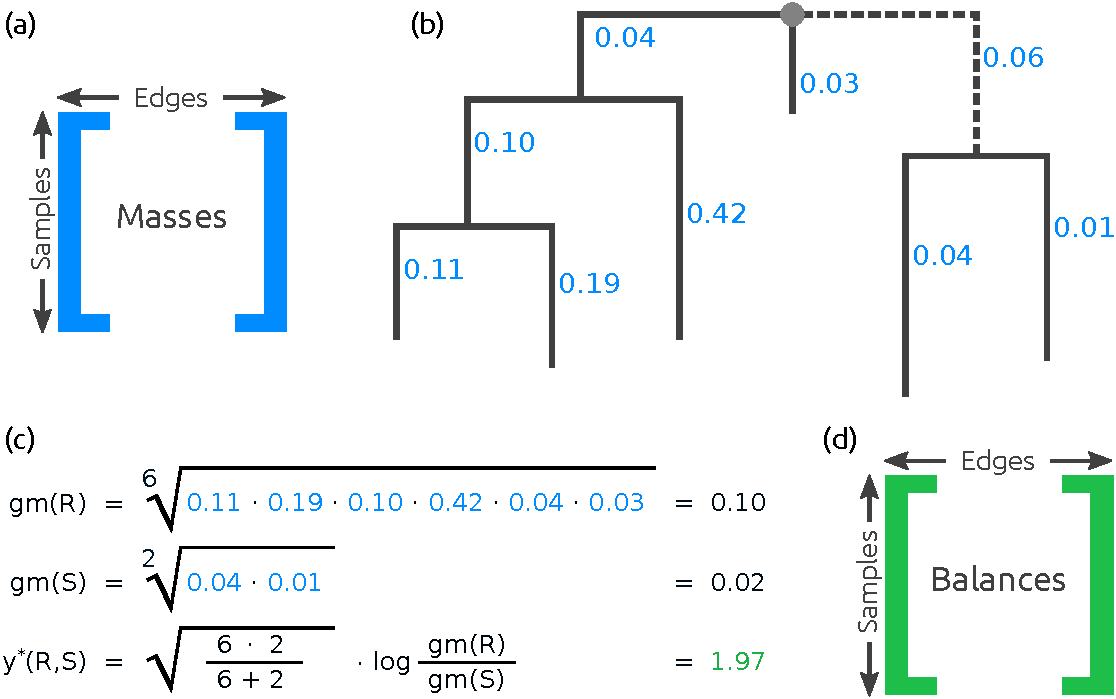
\includegraphics[width=1\linewidth]{pdf/balances.pdf}
    \begin{subfigure}{0pt}
        \phantomcaption
        \label{fig:balances:sub:masses}
    \end{subfigure}
    \begin{subfigure}{0pt}
        \phantomcaption
        \label{fig:balances:sub:tree}
    \end{subfigure}
    \begin{subfigure}{0pt}
        \phantomcaption
        \label{fig:balances:sub:calculation}
    \end{subfigure}
    \begin{subfigure}{0pt}
        \phantomcaption
        \label{fig:balances:sub:balances}
    \end{subfigure}
    \caption[Example computation of the balances between two subtrees]{
        \textbf{Example computation of the balances between two subtrees.}
        \subref{fig:balances:sub:masses}
        The basis of the computation are the per-branch masses of the samples, 
        which are here summarized in the mass matrix, c.\,f. \figref{fig:masses_imbalances:sub:Matrices}.
        \subref{fig:balances:sub:tree}
        We here show the computation of the balance for the two subtrees induced by the dashed edge of the tree,
        for one sample.
        Numbers next to edges are the accumulated per-edge placement masses of the sequences in the sample,
        that is, one row of the matrix.
        We call the left hand side of the tree R, and the right hand side S, as seen from the dashed edge.
        For simplicity, we do not use weighting here; that is, we assume $\bm{p} = ( 1, \ldots, 1 )$.
        \subref{fig:balances:sub:calculation}
        First, the geometric means for both subtrees are calculated, then, their balance.
        The balance is positive, indicating that subtree R contains more placement mass on (geometric) average.
        \subref{fig:balances:sub:balances}
        The compuation is repeated for all edges and for all samples, yielding the \emph{balance matrix} shown here.
    }
    \label{fig:balances}
\end{figure}

% balance can be computed for nodes, subtrees, or -- similar to imbalances, for two sides of an edge.
Balances as defined here can be computed as a measure of \emph{contrast} between any disjoint sets $R$ and $S$ of edges.
Interchanging $S$ and $R$ flips the sign of the balance;
this is irrelevant for the subsequent steps presented here, as long as the interchange is applied consistently.
% We decided for the convention of using the subtree that contains the root for the numerator,
% in accordance with edge imbalances.
When computing the balance between the edges in the two subtrees induced by some given edge $e$,
the conceptual similarity with the previously described edge imbalances 
(\secref{ch:Foundations:sec:PhylogeneticPlacement:sub:PlacementProcessing:par:EdgeImbalances}) becomes apparent:
Imbalances use the difference of sums for contrasting and aggregating,
while balances use the ratio of means for the same purpose.
Hence, balances represent a similar transformation of the placement data,
that can also be used to conduct analyses, such as the Phylofactorization, as presented in \chpref{ch:Factorization}.

We however remark that using (unweighted) balances in our previously presented methods,
such as Edge Correlation (\secref{ch:Visualization:sec:Methods:sub:EdgeCorrelation})
and $k$-means clustering (\secref{ch:Clustering:sec:Methods:sub:PhylogeneticKmeans}),
might lead to spurious results, due to the insensitivity of the geometric mean to singular large values.
That is, individual branches that accumulate a large fraction of the placement mass (sequence abundances)
might only insignificantly change the geometric mean of their clade.
However, such branches are typically the interesting ones,
and hence should exert more influence on the transformation, which is exactly the purpose of the taxon weighting scheme.
This further implies that balances are not indifferent to splittings of reference taxa into multiple representatives
(pers.~comm. with A.~Washburne on 2018-11-23).
%the distribution of placement masses across several branches of related species
% yields different balances compared to having a single representative taxa in the \ac{RT};
We discuss the implications of this in more detail in the evaluation of the method (\secref{ch:Balances:sec:Results}).

% Hence, balances can also be employed for our other methods presented above, such as
% \nameref{sec:MaterialsMethods:sub:Visualization:sub:Correlation} and
% \nameref{sec:MaterialsMethods:sub:Clustering:sub:kmeans}.

% Comparing the per-node balance across samples allows to find nodes that change with respect to the balance,
% indicating ``factors'' that explain differences between the samples in terms of the phylogeny.
% The transformation into balances yields orthogonal components, which are not compositional any more,
% and can hence be used with many standard analysis methods.

% ----------------------------------------------------------------------------------------------------------------------
%     Edge Weights
% ----------------------------------------------------------------------------------------------------------------------

\subsection{Taxon Weighting Scheme}
\label{ch:Balances:sec:Methods:sub:EdgeWeights}

The PhILR also allows for incorporating two distinct weighting schemes for the balances,
one based on taxon abundances, and one based on the branch lengths of the underlying phylogeny \cite{Silverman2017}.
As mentioned above, we implemented the former, while leaving the latter as future work.

We here describe how to adapt the taxon weights of \citeay{Silverman2017} to our placement-based approach,
that is, how an appropriate vector $\bm{p}$ of taxon weights for the edges can be constructed.
Originally, this taxon weighting scheme down-weighs the influence of low abundant taxa \cite{Silverman2017},
which are known to be less reliable and more variable \cite{Good1956}.
Here, we accordingly down weigh edges with low placement mass, for the same reasons.
We follow the approach of \citeay{Silverman2017}, and construct the taxon weights by multiplicatively combining two terms:

\begin{enumerate}
    \item A measure for the central tendency of the absolute edge masses, for example, their mean across all samples.
          This is the main component of the weight that yields low values for edges with low mass and vice versa.
    \item A vector norm of the relative edge masses across the samples.
          This term additionally weighs edges by their specificity.
\end{enumerate}

Our implementation allows to use the median, the arithmetic mean, and the geometric mean,
as well as different $\ell_p$-norms (such as the Manhattan, Euclidean, and maximum norm),
and the Aitchison norm \cite{Pawlowsky-Glahn2015}.
We follow the advice of \cite{Silverman2017}, and by default use the geometric mean
(with pseudo-counts added to the masses to avoid skew from edges without any placement mass) and the Euclidean norm.
In that case, the weights for edge $j$ are computed as follows:

\begin{equation}
    \label{ch:Balances:sec:Methods:eq:EdgeWeights}
%     p_j = \sqrt[n]{ ( c_{j1} + 1 ) \cdot \ldots \cdot ( c_{jn} + 1 ) } \cdot \| x_j \|
%     p_j ~=~ \sqrt[n]{ \prod_{i=1}^{n} ( \tilde{c}_{ji} + 1 ) }  ~\cdot~  \| \tilde{x}_j \|_2
    p_j ~=~ \sqrt[n]{ \prod_{i=1}^{n} ( \tilde{c}_{ji} + 1 ) }  ~~\cdot~  \sqrt{ \sum_{i=1}^{n} \tilde{x}_{ji}^2 }
\end{equation}

Here, $n$ is the number of samples, $\tilde{c}_j$ is the vector of absolute masses at edge $j$ across all samples,
and $\tilde{x}_j$ the vector of relative masses at edge $j$ across all samples, both of length $n$.
That is, these measures use the masses of all $n$ samples;
consequently, we here use columns instead of rows of the edge masses matrix of \figref{fig:balances:sub:masses}
(which is identical to \figref{fig:masses_imbalances:sub:Matrices}),
where each column is used for the weights of the corresponding edge.
The resulting taxon weights $\bm{p}$ are then fixed and used across the balance computation of all samples.

% this corresponds to taxon weights of \cite{Silverman2017}.
% as we consider masses on edges instead of abundances at the tips of the tree, we use the term edge weights instead of taxon weights here.
% note that these weights are meant as a weighting mechanism to reduce the influence of low abundance taxa / edges with low mass.
% the terms weight and mass should not be confused here!

% ######################################################################################################################
%         Evaluation and Results
% ######################################################################################################################

\section{Evaluation and Results}
\label{ch:Balances:sec:Results}

As a first test of our adaptation of balances to placement data, we apply it to the \ac{BV} dataset \cite{Srinivasan2012}.
Further assessment of balances for placement data, also with the \ac{HMP} dataset \cite{Huttenhower2012,Methe2012},
is implicitly conducted by the evaluation of Placement-Factorization in \secref{ch:Factorization:sec:Evaluation},
which uses balances for aggregation and contrasting of subtrees.
% We hence refrain here from further tests.
See \appref{supp:sec:DetailsEmpiricalDatasets:sub:BV} and \appref{supp:sec:DetailsEmpiricalDatasets:sub:HMP}
for descriptions of the datasets.

% ----------------------------------------------------------------------------------------------------------------------
%     Principal Components
% ----------------------------------------------------------------------------------------------------------------------

\subsection{Principal Components}
\label{ch:Balances:sec:Results:sub:PrincipalComponents}

As balances are conceptually similar to edge imbalances, we perform analogous evaluations.
To this end, we computed the per-edge balance for all edges of the \ac{BV} reference tree, across all \num{220} samples.
That is, for each edge, we computed the balance between the two subtrees induced by the edge.
This yields the \emph{balance matrix}, as shown in \figref{fig:balances:sub:balances},
which corresponds to the imbalance matrix used for Edge PCA, c.\,f. \figref{fig:masses_imbalances:sub:Matrices}.
Hence, a natural first visualization of the balances is to analyze their principal components,
that is, to compute the PCA of the balance matrix.
The first two components of the \ac{BV} balances are shown in \figref{fig:bv_place_edge_balances_pca_scatter},
for both variants of the balance computation (with and without taxon weighting).
% The principal components exhibit a separation of the samples by Nugent score,
% showing that they yield results comparable to Edge PCA.
% In order to interpret what the axes of these principal components mean,
Furthermore,
we can again employ the visualization of PCA eigenvectors on the reference tree as used in Edge PCA \cite{Matsen2011a}.
% c.\,f., \figref{fig:epca}.
We show the results for %PCA on the balances of 
the \ac{BV} dataset in \figref{fig:bv_place_edge_balances_pca_trees},
where we visualize the first two principal components of the balances with and without taxon weighting on the tree.
% The figure shows the edges that are responsible for the splits seen in \figref{fig:bv_place_edge_balances_pca_scatter}.

\begin{figure}[!htb]
    \centering
    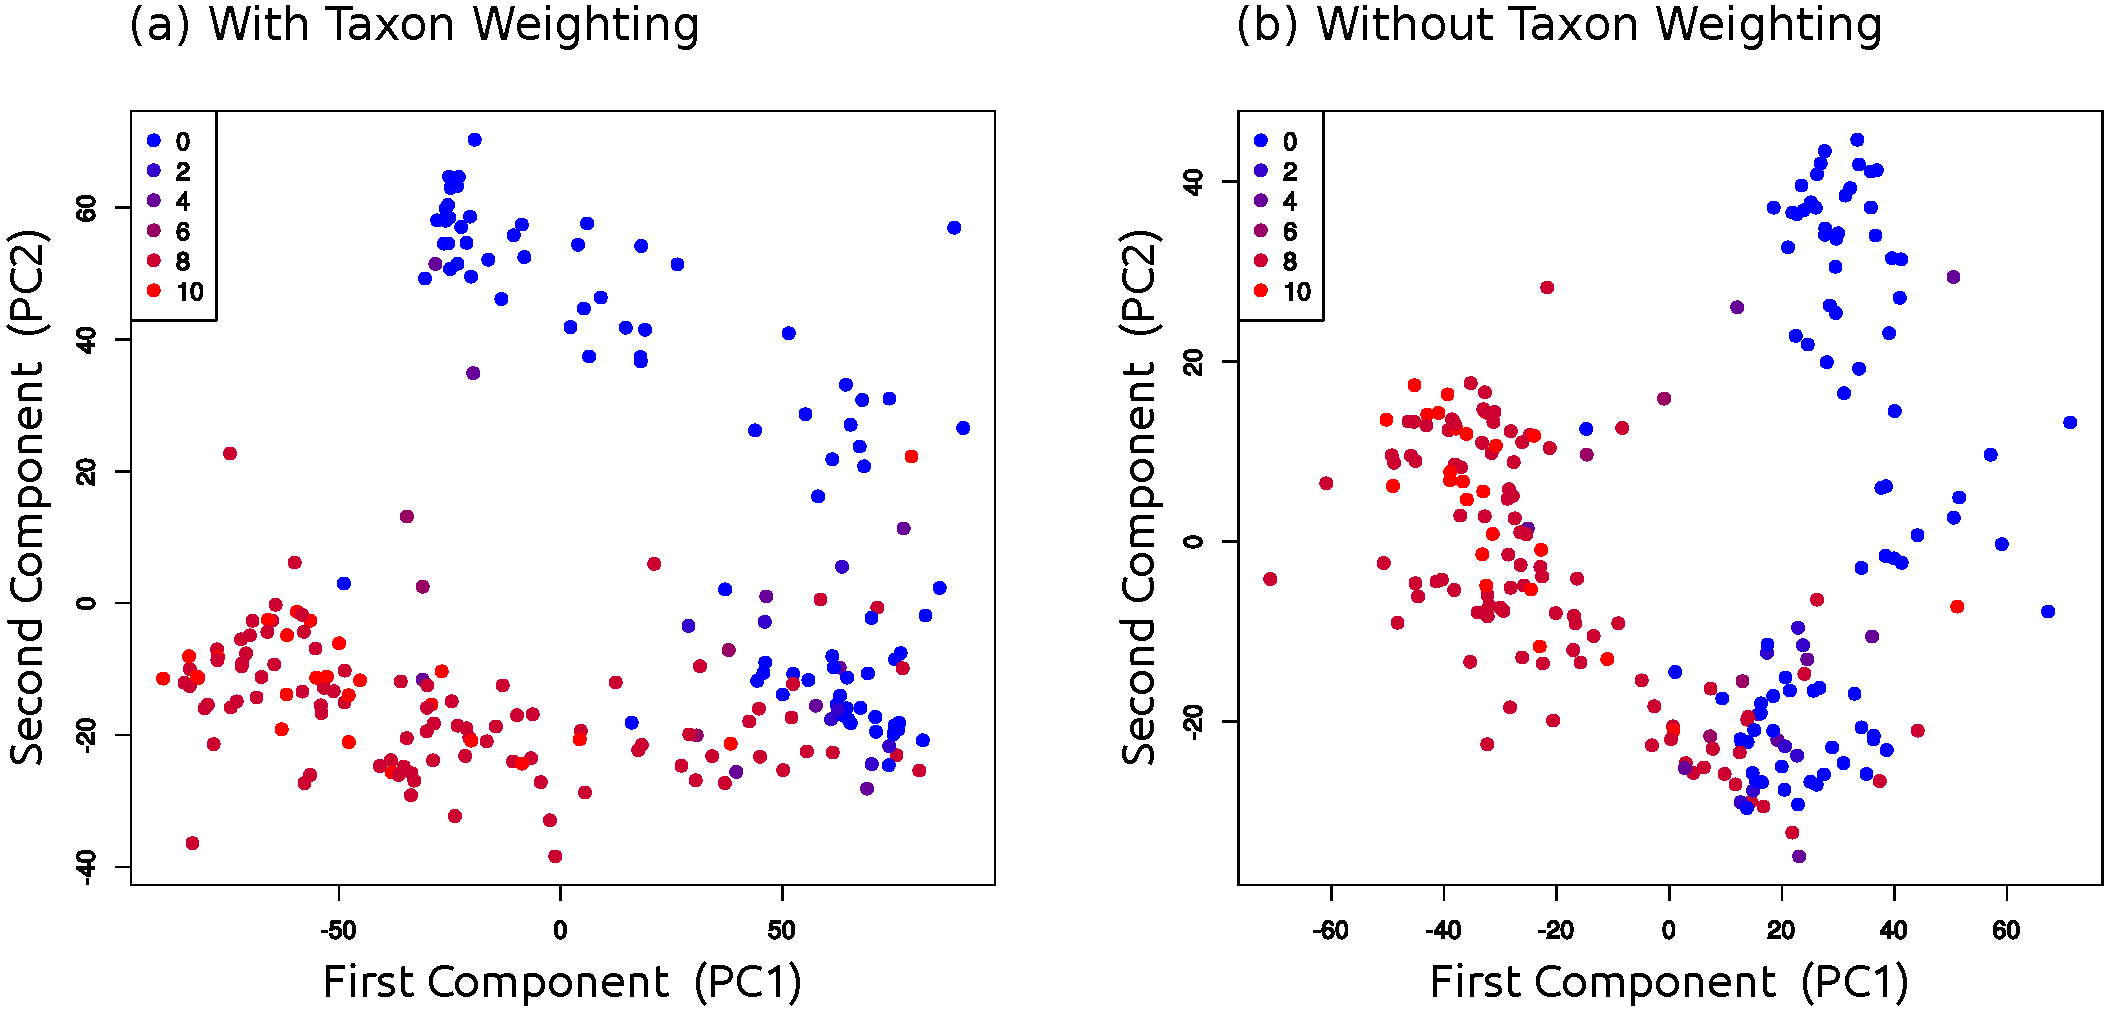
\includegraphics[width=\linewidth]{pdf/bv_place_edge_balances_pca_scatter.pdf}
    \begin{subfigure}{0pt}
        \phantomcaption
        \label{fig:bv_place_edge_balances_pca_scatter:sub:with_taxon_weighting}
    \end{subfigure}
    \begin{subfigure}{0pt}
        \phantomcaption
        \label{fig:bv_place_edge_balances_pca_scatter:sub:without_taxon_weighting}
    \end{subfigure}
    \caption[Projection of edge balance PCA components of the \acs{BV} dataset]{
        \textbf{Projection of edge balance PCA components of the \ac{BV} dataset.}
        The plots show the first two principal components of a PCA on the per-edge balances,
        calculated on placements of the data on reference tree of the \ac{BV} dataset.
        That is, for each edge of the tree, we calculated the balance (log-ratio of geometric means)
        of the placement masses of the \ac{BV} samples between the two sides of the tree induced by the edge.
        Then, we computed a PCA on the resulting balance matrix.
        \subref{fig:bv_place_edge_balances_pca_scatter:sub:with_taxon_weighting} shows the result when
        using taxon weighting \cite{Silverman2017} in the balances calculation,
        while \subref{fig:bv_place_edge_balances_pca_scatter:sub:without_taxon_weighting} shows the result
        without taxon weighting.
        Each item represents a sample, colored by its Nugent score (0 means healthy, 10 means severe illness);
        the Nugent score had no influence on the PCA calculations.
    }
    \label{fig:bv_place_edge_balances_pca_scatter}
\end{figure}

\begin{figure}[!phtb]
    \centering
    \includegraphics[width=\linewidth]{pdf/bv_place_edge_balances_pca_trees.pdf}
    \begin{subfigure}{0pt}
        \phantomcaption
        \label{fig:bv_place_edge_balances_pca_trees:sub:tw_pc1}
    \end{subfigure}
    \begin{subfigure}{0pt}
        \phantomcaption
        \label{fig:bv_place_edge_balances_pca_trees:sub:tw_pc2}
    \end{subfigure}
    \begin{subfigure}{0pt}
        \phantomcaption
        \label{fig:bv_place_edge_balances_pca_trees:sub:no_tw_pc1}
    \end{subfigure}
    \begin{subfigure}{0pt}
        \phantomcaption
        \label{fig:bv_place_edge_balances_pca_trees:sub:no_tw_pc2}
    \end{subfigure}
    \caption[Eigenvectors of edge balance PCA of the \acs{BV} dataset]{
        \textbf{Eigenvectors of edge balance PCA of the \ac{BV} dataset.}
        The figure shows the eigenvectors of the first two principal components of PCA
        on the per-edge balances with and without taxon weighting,
        visualized on the reference tree of the \ac{BV} dataset.
%         See \figref{fig:bv_place_edge_balances_pca_scatter} for details on the balances calculation.
        The visualization of the components on the reference tree is analogous
        to the Edge PCA tree visualization as for example shown in \figref{fig:epca}.
        As the data that is considered in the PCA corresponds to the edges of the tree,
        the resulting eigenvectors can be mapped back onto the tree, which is shown here.
        Each edge is colored according to the corresponding value of the first principal component
        in \subref{fig:bv_place_edge_balances_pca_trees:sub:tw_pc1}
        and \subref{fig:bv_place_edge_balances_pca_trees:sub:no_tw_pc1},
        and the second principal component
        in \subref{fig:bv_place_edge_balances_pca_trees:sub:tw_pc2}
        and \subref{fig:bv_place_edge_balances_pca_trees:sub:no_tw_pc2}, respectively.
        In \subref{fig:bv_place_edge_balances_pca_trees:sub:tw_pc1}
        and \subref{fig:bv_place_edge_balances_pca_trees:sub:no_tw_pc1},
        we marked the \taxonname{Lactobacillus crispatus} clade with a black arc at the left of the tree.
    }
    \label{fig:bv_place_edge_balances_pca_trees}
\end{figure}

\figref{fig:bv_place_edge_balances_pca_trees} hence indicates how the axes of the principal components
in the PCA scatter plots of \figref{fig:bv_place_edge_balances_pca_scatter} can be interpreted:
The first component leads to the \taxonname{Lactobacillus} clade,
while the second one splits this clade into \taxonname{Lactobacillus iners} and \taxonname{Lactobacillus crispatus}.
Both plots of \figref{fig:bv_place_edge_balances_pca_scatter} separate the healthy from the sick patients.
However, in contrast to Edge PCA, the first component of
\figref{fig:bv_place_edge_balances_pca_scatter:sub:with_taxon_weighting}
does not fully distinguish between the healthy (blue) and diseased (red) samples.
For yet to explore reasons, the component only takes \taxonname{Lactobacillus iners} into account,
while mostly ignoring \taxonname{Lactobacillus crispatus}.
This can be seen in \figref{fig:bv_place_edge_balances_pca_trees:sub:tw_pc1},
which shows the eigenvectors of this component visualized on the reference tree.
There, the path leading to the \taxonname{Lactobacillus} clade
does not include the branches of \taxonname{Lactobacillus crispatus}, which is marked with a black arc.
Including the second component however, which distinguishes between the two types of \taxonname{Lactobacillus},
as shown in \figref{fig:bv_place_edge_balances_pca_trees:sub:tw_pc2},
yields a clear separation of the samples.
On the other hand, \figref{fig:bv_place_edge_balances_pca_scatter:sub:without_taxon_weighting}
exhibits closer similarities to the Edge PCA plot shown in \figref{fig:kmeans_all:sub:epca_ns},
in that the first component separates healthy from sick,
and the second component further splits the healthy individuals apart.
% In fact, the only difference to Edge PCA is the use of balances instead of imbalances for the PCA.

Hence, the results obtained from this analysis are consistent with our previous findings, in particular with Edge PCA.
% c.\,f., \figref{fig:epca} and \cite{Srinivasan2012}.
% in order to show that balances without taxon weighting do not include this clade in the first component.
The principal components separate the samples by Nugent score,
with the first component mostly separating \taxonname{Lactobacillus} from the rest of the tree,
and the second component further distinguishing
between \taxonname{Lactobacillus crispatus} and \taxonname{Lactobacillus iners}.

% showing that they yield results comparable to Edge PCA.
% As with Edge PCA, the principal components correspond to the \taxonname{Lactobacillus} clade,

% ----------------------------------------------------------------------------------------------------------------------
%     Edge Correlation
% ----------------------------------------------------------------------------------------------------------------------

\subsection{Edge Correlation}
\label{ch:Balances:sec:Results:sub:EdgeCorrelation}

As mentioned in the method description (\secref{ch:Balances:sec:Methods:sub:ILRTransform}),
balances could in principle be used as input to our previously presented methods,
such as Edge Correlation and $k$-means clustering (which adequately might be called Balance $k$-means),
in the same manner that we used imbalances in these methods.
To provide an example of using balances with these methods, 
we show the correlation of the Nugent score with balances in \figref{fig:bv_place_edge_balances_correlation}.

\begin{figure}[!htb]
    \centering
    \includegraphics[width=\linewidth]{pdf/bv_place_edge_balances_correlation.pdf}
    \begin{subfigure}{0pt}
        \phantomcaption
        \label{fig:bv_place_edge_balances_correlation:sub:with_taxon_weighting}
    \end{subfigure}
    \begin{subfigure}{0pt}
        \phantomcaption
        \label{fig:bv_place_edge_balances_correlation:sub:without_taxon_weighting}
    \end{subfigure}
    \caption[Correlation of the edge balances of the \acs{BV} dataset with Nugent score]{
        \textbf{Correlation of the edge balances of the \ac{BV} dataset with Nugent score.}
        The Edge Correlation method as presented in \secref{ch:Visualization:sec:Methods:sub:EdgeCorrelation},
        and for example shown in \figref{fig:all_nugent},
        can also be conducted using balances (instead of masses or imbalances).
        We here show Edge Correlation using Spearman's Rank Correlation Coefficient,
        calculated on the per-edge balances and the Nugent score, based on the placement of the \ac{BV} dataset.
        That is, for each edge of the tree, we calculated the balance (log-ratio of geometric means)
        of the placement masses of the \ac{BV} samples between the two sides of the tree induced by the edge.
        Then, we calculated the correlation with the Nugent score of each sample, and visualized it on the tree.
        \subref{fig:bv_place_edge_balances_correlation:sub:with_taxon_weighting} shows the result when
        using taxon weighting \cite{Silverman2017} in the balances calculation,
        while \subref{fig:bv_place_edge_balances_correlation:sub:without_taxon_weighting} shows the result
        without taxon weighting.
    }
    \label{fig:bv_place_edge_balances_correlation}
\end{figure}

The result of this balance-based Edge Correlation with taxon weighting,
shown in \figref{fig:bv_place_edge_balances_correlation:sub:with_taxon_weighting},
is similar to the correlation with imbalances in \figref{fig:all_nugent:sub:srcc_ei}:
An anti-correlation with the \taxonname{Lactobacillus} clade is again visible
(less placement mass in this clade means higher Nugent score, that is, indicates a more severe illness),
while several other clades exhibit a positive correlation with Nugent score.
Hence, balance-based Edge Correlation \emph{with} taxon weighting is consistent with our previous findings,
and with the imbalance-based variant of this method.

However, artifacts might arise from the underlying mathematical framework of balances,
in particular the usage of the geometric mean \emph{without} taxon weighting:
The geometric mean is \emph{not} sensitive to singular large values,
such as the high amount of placement mass on one of the \taxonname{Lactobacillus} branches.
It only significantly increases if multiple high values are present,
such as the multitude of bacterial taxa with high abundance in diseased patients of the \ac{BV} dataset \cite{Srinivasan2012}.
This can lead to spurious results, as shown in
\figref{fig:bv_place_edge_balances_correlation:sub:without_taxon_weighting},
where the correlation of the unweighted balances %without taxon weighting
with the Nugent score yields unrealistically high negative correlations
for almost all branches that have little placement mass on them (red branches).

%         However, as mentioned in the main text, without taxon weighting, spurious results can occur.
% The most striking difference to the previous Edge Correlation trees in \figref{fig:all_nugent}
% is however the majority of spuriously anti-correlated (red) edges in the tree \emph{without} taxon weighting
% in \figref{fig:bv_place_edge_balances_correlation:sub:without_taxon_weighting}.
% As mentioned in the method description in \secref, this is due to the insensitivity of the geometric mean
% to the presence of singular large values:
The reason that the insensitivity of the geometric mean to the presence of singular large values
leads to the majority of spuriously anti-correlated edges is as follows:
If most values are small, so will be their geometric mean, even if a few very large values are also present.
As can be seen in \figref{fig:heat_tree} and \figref{fig:all_dispersions},
the clades that exhibit a high anti-correlation (red) in \figref{fig:bv_place_edge_balances_correlation:sub:without_taxon_weighting}
have low placement mass with a low variance.
Hence, the geometric mean of the masses in these clades is consistently low across samples,
which means that the numerator of the log-ratio in the balances computation has little effect on the correlation.
This implies that the denominator, which represents the rest of the tree,
drives the anti-correlations seen in \figref{fig:bv_place_edge_balances_correlation:sub:without_taxon_weighting}.
Women affected by \ac{BV} show a presence of several different bacterial clades,
while healthy women without \ac{BV} almost exclusively have high presence
of one of two types of \taxonname{Lactobacillus} \cite{Srinivasan2012}.
Hence, in samples with \ac{BV} (high Nugent score), there are several distinct edges that have an elevated mass,
which is enough to change the geometric mean,
while in samples without \ac{BV} (low Nugent score),
most of the mass is concentrated on a single edge of the \taxonname{Lactobacillus} clade,
which is not enough to significantly change the geometric mean.
In consequence, the denominator of the balance at the spurious edges is consistently larger
for samples with \ac{BV} compared to those without \ac{BV}.
Thus, the balance is smaller for samples with a high Nugent score,
which finally explains the observed anti-correlations.
Note that despite this, there are still edges that exhibit positive correlation (blue and green),
which is where the actual patterns in the data outweigh the insensitivity of the geometric mean.

Lastly, this property of insensitivity of the geometric mean implies that it \emph{is} sensitive to taxa splitting,
that is, to the number of reference sequences that a taxon or species is represented by in the reference tree
(pers.~comm. with A.~Washburne on 2018-11-23):
For example, in the context of balances of phylogenetic placements,
it \emph{does} make a difference whether masses are focused on a single branch,
or distributed across several representatives of the same species.
Hence, in summary,
we do not recommend to use (unweighted) balances for computations such as correlations or $k$-means clustering.

% ######################################################################################################################
%         Summary and Outlook
% ######################################################################################################################

\section{Summary and Outlook}
\label{ch:Balances:sec:SummaryOutlook}

In this chapter, we introduced an adaptation of the Phylogenetic ILR transform and balances \cite{Silverman2017}
to phylogenetic placements.
Balances are conceptually similar to edge imbalances, exhibit similar properties, 
and can be used for similar types of analyses.
% hence combining previously existing concepts from different 
% of OTU-based balances with placement-based edge imbalances.
Hence, with this adaptation, we helped to bridge the methodological gap
between OTU-based and placement-based approaches to analysing metagenomic data.
This might lead to future development of novel methods and adaptations,
with the intention of obtaining a better, more complete picture of metagenomic data,
by combining the strengths of both the OTU-based and the placement-based approaches.

As balances are a transformation that yields orthogonal components (one for each node or branch of the tree),
issues pertaining to the normalization of compositional data do not arise.
With samples being represented as a vector of balances,
numerous standard tools for data visualization, ordination, and clustering in the Euclidean space
can be readily applied to phylogenetic placement data.
Applying these methods to placements instead of OTUs allows for more detailed analyses,
as the entire original sequence data can be used.
Furthermore, using a fixed reference tree instead of one inferred from the OTUs present in a set of samples
enables comparative studies across datasets.

A drawback of both balances and imbalances in the context of phylogenetic placements
is that the edges leading to tips of the reference tree do not have meaningful values.
This is because they measure differences between masses on the two sides of the edge
(of which tip edges only have one), while ignoring the mass on the respective edge itself.
For most forms of analysis, this does not pose a concerning issue, as the trees are usually large enough
to have enough edges that can be used in the downstream steps.
% In particular in cases where the tree contains several strains from the same species,
% the tip edges do not carry much information anyway.
% We note however that this might also have effects on the quality of the placements themselves,
% for example in terms of their likelihood weight ratios, which might be distributed across the tips,
% leading to a blurred signal in the analyses.
Still, we see potential for future improvement of the concepts of balances and imbalances
by expanding their definition to also yield meaningful values for tip edges.
A simple approach for example would be to declare all placement mass on an edge
to be on the distal (away from the root) side of the edge.
We however did not assess the implications of this approach for the mathematical consistency of the methods yet.

In the context of this work, balances are used as an intermediary tool
in order to describe a set of samples in the context of a reference tree.
In this chapter, we evaluated some basic analysis and visualization techniques in order to show
that balances yield consistent results on empirical datasets compared to concepts such as edge imbalances.
In the following chapter, we introduce Placement-Factorization,
which uses balances as a description of clades of the reference tree.
